$subject$=Физические основы компьютерных \\ и сетевых технологий
$teacher$=Решение задач из сборника
$date$=

\clearpage

\begin{tcolorbox}
    \textbf{Задача 2.3.8.} Две длинные параллельные нити равномерно
    заряжены с одинаковой линейной плотностью заряда $\tau$. Найти
    максимальное значение модуля напряженности поля в плоскости
    симметрии этой системы. Расстояние между нитями $d$.
\end{tcolorbox}

\begin{minipage}{\textwidth}
    \begin{wrapfigure}{r}{0pt}
        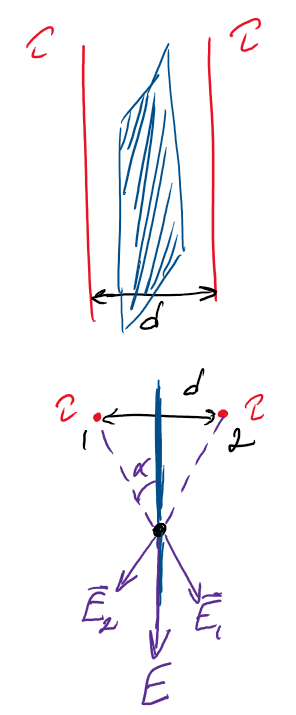
\includegraphics[width=0.35\textwidth]{physics1/images/physics1_homework_7_1}
    \end{wrapfigure}

    Будем считать нити бесконечно длинными. Тогда известна напряженности заряженной нити до точки на расстоянии $r$: $\frac{2k\tau}{r}$

    В точке между нитями в силу симметрии напряженность равна по модулю и противоположна по напрявлению. Найдем напряженность в точке,
    отрезки от которой до одной из нитей и середины между нитями образуют угол $\alpha$. В силу симметрии, напряженности
    каждой нити в точке равны:

    $|\vec{E}_1| = |\vec{E}_2| = 2k\tau \frac{2\sin\alpha}{d}$

    Спроецируем эти вектора на плоскость симметрии:

    $|\vec{E}| = 2\cos\alpha |\vec{E}_1| = \frac{8k\tau \sin\alpha\cos\alpha}{d} = \frac{4k\tau \sin2\alpha}{d}$

    Получаем, что $|\vec{E}|$ принимает наибольшее значение при $\sin2\alpha = 1 \Longrightarrow \alpha = \frac{\pi}{4}$

    В этом случае $|\vec{E}| = \frac{4k\tau}{d}$
\end{minipage}

\bigvspace

\underline{Ответ}: $\frac{4k\tau}{d}$


\clearpage

\begin{tcolorbox}
    \textbf{Задача 3.3.5.} Два коаксиальных кольца одинакового радиуса $R$
    заряжены равномерно зарядами $q_1$ и $q_2$. Плоскости колец находятся
    на расстоянии $h$ друг от друга. Найти потенциал в произвольной
    точке $A$ на оси колец.
\end{tcolorbox}

\begin{minipage}{\textwidth}
    \begin{wrapfigure}{r}{0pt}
        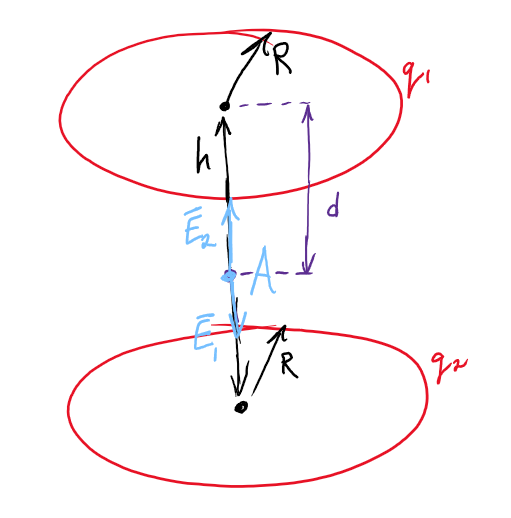
\includegraphics[width=0.4\textwidth]{physics1/images/physics1_homework_7_2}
    \end{wrapfigure}

    Пусть точка находится на расстоянии $d$ от первого кольца. Найдем формулу потенциал в этой точки

    Очевидно, что потенциал на бесконечном расстоянии от точки можем считать равным нулю (тогда считаем кольцо точечным зарядом). 

    Тогда $\varphi_A - \varphi_\infty = \int_{d}^{\infty} \vec{E}d\vec{l} = \int_{d}^{\infty} \frac{kqr}{\sqrt{R^2 + r^2}} dr = 
    -\frac{kq}{\sqrt{R^2 + r^2}} \Big|_{d}^{\infty} = \frac{kq}{\sqrt{R^2 + d^2}}$

    В нашем случае по принципу суперпозиции потенциал в точке $A$ равен $\varphi = \varphi_1 + \varphi_2 = 
    \frac{kq}{\sqrt{R^2 + d^2}} + \frac{kq}{\sqrt{R^2 + (h - d)^2}} = 
    kq\left(\frac{\sqrt{R^2 + d^2} + \sqrt{R^2 + (h - d)^2}}{\sqrt{(R^2 + d^2)(R^2 + (h - d)^2)}}\right)$
\end{minipage}

\bigvspace

\underline{Ответ}: $\frac{kq}{\sqrt{R^2 + d^2}} + \frac{kq}{\sqrt{R^2 + (h - d)^2}}$

\clearpage

\begin{tcolorbox}
    \textbf{Задача 1.10.} Потенциал поля внутри заряженного шара зависит только от
    расстояния $r$ до его центра по закону $\varphi = ar^2 + b$, где $a$ и $b$ — постоянные. 
    Найти распределение объемного заряда $\rho(r)$ внутри
    шара.
\end{tcolorbox}

\begin{minipage}{\textwidth}
    \begin{wrapfigure}{r}{0pt}
    \end{wrapfigure}

    По уравнению Пуассона:

    $-\Delta \varphi = \frac{\rho}{\varepsilon_0}$

    В нашем случае $-\Delta \varphi = -\vec\nabla\vec\nabla(ar^2 + b) = -\vec\nabla\vec\nabla(a(x^2 + y^2 + z^2) + b) = 
    -\vec\nabla\left(2ax\vec{i} + 2ay\vec{j} + 2az\vec{k}\right) = -2a - 2a - 2a = -6a$

    Из этого $\rho(r) = -\Delta \varphi \varepsilon_0 = -6a\varepsilon_0$
\end{minipage}

\bigvspace

\underline{Ответ}: $-6a\varepsilon_0$


\begin{tcolorbox}
    \textbf{Задача 15.47.} Тонкий стержень согнут в кольцо радиусом $R = 10$ см.
    Он заряжен с линейной плотностью $\tau = 300$ нКл/м. Какую работу
    $A$ надо совершить, чтобы перенести заряд $Q = 5$ нКл из центра кольца в точку,
    расположенную на оси кольца на расстоянии $l = 20$ см от центра его?
\end{tcolorbox}


\begin{minipage}{\textwidth}
    \begin{wrapfigure}{r}{0pt}
        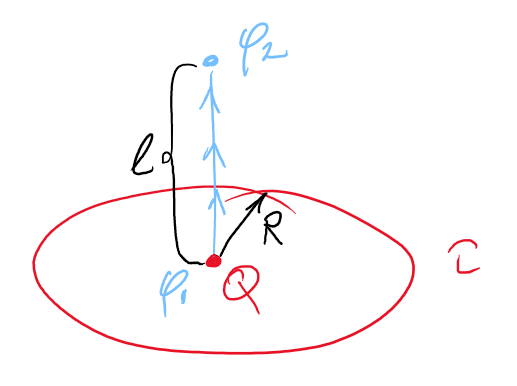
\includegraphics[width=8cm]{physics1/images/physics1_homework_7_3}
    \end{wrapfigure}

    Из лекций знаем, что работа по перемещению заряда равна произведению величины заряда на разность потенциалов: 
    $A = Q\Delta\varphi$

    Потенциал поля кольца в точке на оси равен $\varphi(r) = \frac{kq_{\text{кольца}}}{\sqrt{R^2 + r^2}}$

    Тогда $\varphi_1 = \frac{kq_{\text{кольца}}}{R}$, а $\varphi_2 = \frac{kq_{\text{кольца}}}{\sqrt{R^2 + l^2}}$

    $q_{\text{кольца}} = \tau \cdot 2\pi R$

    Тогда работа равна 
    
    $A = Q\Delta \varphi = Q(\varphi_1 - \varphi_2) = 
    Q\left(\frac{kq_{\text{кольца}}}{R} - \frac{kq_{\text{кольца}}}{\sqrt{R^2 + l^2}}\right) = 
    Qk\tau \cdot 2\pi R \left(\frac{1}{R} - \frac{1}{\sqrt{R^2 + l^2}}\right) = 
    Qk\tau \cdot 2\pi \left(1 - \frac{R}{\sqrt{R^2 + l^2}}\right) = 4.689 \cdot 10^{-5}$ Дж

\end{minipage}

\bigvspace

\underline{Ответ}: $4.689 \cdot 10^{-5}$ Дж

